\documentclass[oneside,reqno,letterpaper]{amsart}

\usepackage{silence} % for suppressing warnings
\WarningFilter{mdframed}{You have requested package}

\usepackage[workingpaper]{/Users/aden/Library/CloudStorage/Box-Box/latex/adenc}
\raggedbottom

\usepackage{biblatex}
\addbibresource{ref.bib}


% ========== newcommand ==========
% weak star convergence:
\newcommand{\weakto}{\rightharpoonup}
\newcommand{\weakstarto}{\stackrel{\ast}{\rightharpoonup}}

\newcommand{\stronglim}{\text{s-lim}}

% spectral theory
\newcommand{\pspec}{\spec_{\mathrm{p}}}
\newcommand{\discspec}{\spec_{\text{disc}}}
\newcommand{\essspec}{\spec_{\text{ess}}}

% ========== fonts ==========
\usepackage{newtxtext}
\usepackage{newtxmath}
% \renewcommand{\familydefault}{\sfdefault}
% \usepackage{cmbright}


% \setcounter{tocdepth}{1}




\title[Spectral Theory and the Min-Max Theorem]{Spectral Theory and the Min-Max Theorem}
\author{Aden Chen}


\begin{document}

\begin{abstract}
  The min-max theorem offers a variational characterization of the discrete eigenvalues that lie below the essential spectrum of a self-adjoint operator. 
  In this paper, we develop the necessary tools and present a proof of this theorem. 
\end{abstract}

\maketitle

\tableofcontents




\section*{Introduction}
This paper offers a brief introduction to spectral theory, covering key concepts such as the spectrum, resolvent, functional calculus, and spectral projections, and ultimately proving the min-max theorem. 

\Cref{sec:hilbert} reviews the concept of Hilbert spaces and their structures. 
\Cref{sec:operators} introduces the adjoint, unitarity, and closure, and presents the multiplication operator. 
We then define the spectrum and resolvent set in \Cref{sec:spectrum-resolvent}, discussing their properties and calculating the spectra of different sets of operators. 
These foundations are essential for \Cref{sec:spectral-thm}, where we prove the spectral theorem and, along the way, construct a functional calculus.
% ---a method of applying functions defined on the real line to self-adjoint operators.
This leads to the definition of spectral projectors and a discussion on the discrete and essential spectrum in \Cref{sec:spectral-projectors}. 
Finally, in \Cref{sec:min-max}, we prove the min-max theorem. 

We assume the reader is familiar with analysis in \(\RR^n\). 
% Results from real analysis will be used without mention. 
% Basic functional analysis will be occasionally used, but references will always be provided. 






  
\section{Hilbert Spaces}
\label{sec:hilbert}


Recall that a Hilbert space is an inner product space that is complete with respect to the metric induced by its inner product.
We assume that the inner product is linear in the first variable and conjugate linear in the second. 
In what follows, we use the symbol \(\cH\) to denote a separable complex Hilbert space, 
that is, a complex Hilbert space that admits a countable dense subset.


One fundamental property of Hilbert spaces is that every closed subspace admits a complement. 
That is, 

\begin{theorem}
\label{thm:hilbert-direct-sum}
  Let \(M\) be a closed subspace of a Hilbert space \(\cH\). Then \(H = M \oplus M^\perp\). 
\end{theorem}
% This can be proved, for example, using Corollary 5.4 in \cite[p.~134]{brezis2011functional}
\begin{proof}
  See \cite[pp.~137--138, Remark 5]{brezis2011functional}. 
\end{proof}

In fact, this property characterizes Hilbert spaces: a Banach space \(X\) is isomorphic to a Hilbert space if and only if every closed subspace of \(X\) is complemented \cite[p.~39]{brezis2011functional}. 


We start with two consequences of this theorem concerning orthogonal complements and density of subspaces. 
They will be important when dealing with unbounded linear operators, frequently defined only on a dense linear subspace for reasons that will become clear. 


\begin{proposition}
\label{thm:dense-subset-condition}
  Let \(M \subset \cH\). 
  % Let \(\cH\) be a Hilbert space and \(M \subset H\) a nonzero subset. 
  Then \(\Span M\) is dense in \(\cH\) if and only if \(M^\perp = \{0\}\). 
\end{proposition}
\begin{proof}
  Let \(x \in M^{\perp}\) with \(\Span M\) dense in \(\cH\). Thus there exists a sequence \((x_{n})\) in \(\Span M\) converging to \(x\). 
  By continuity of the inner product, \(0 = \left< x_{n}, x \right> \to \left< x, x \right>\) and we have \(x = 0\).
  Conversely, if \(M^{\perp} = \{0\}\), then a fortiori \((\overline{\Span M})^{\perp} = \{0\}\). Since \(\Span M\) is a subspace of \(\cH\), \Cref{thm:hilbert-direct-sum} yields \(H = \overline{\Span M}\). 
\end{proof}


\begin{proposition}
\label{thm:double-perp}
  Let \(W \subset \cH\) be a linear subspace. 
  % Let \(\cH\) be a Hilbert space and \(W \subset \cH\) a linear subspace. 
  Then \((W^\perp)^\perp = \overline{W}\). 
\end{proposition}
\begin{proof}
  By unwrapping the definition, we have \(W \subset (W^\perp)^\perp\). 
  Since \((W^\perp)^\perp\) is closed, the inclusion can be extended to \(\overline{W} \subset (W^\perp)^\perp\) by continuity of the inner product. 
  To prove the opposite inclusion, let \(x \in (W^\perp)^\perp\) be arbitrary and suppose \(x \not\in \overline{W}\). 
  By the Hahn-Banach theorem\footnote{See, e.g., \cite[Chapter 1]{brezis2011functional} or REU paper \cite{peng2014hahn}. }, there exists a continuous linear functional \(f\) on \(\cH\) that strictly separates \(x\) and \(\overline{W}\).
  That is, \(f(w) = 0\) for all \(w \in \overline{W}\) and \(f(x) \neq 0\). 
  Let \(v_f \in \cH\) be the Riesz representation of \(f\) (see \Cref{thm:riesz-representation}) and we have 
  \[
    \left< v_f, w \right> = 0, \quad \forall w \in W . 
  \] 
  So \(v_f \in W^\perp\). 
  But from \(x \in (W^\perp)^\perp\) we know \(\left< v_f, x \right> = 0\), contradicting \(f(x) \neq 0\). 
\end{proof}


Recall, next, the direct sum of Hilbert spaces:
\begin{definition}
  For the sequence of Hilbert spaces \(\{\cH_j\}_{j \in \NN}\), we define their direct sum as 
  \[
    \bigoplus_{j = 1}^{\infty} \cH_j 
    \coloneqq \left\{ (u_1, u_2, \cdots ): u_j \in \cH_j, \sum \norm{u_j}_{\cH_j}^2 < \infty \right\} . 
  \] 
\end{definition}

The assumption on norms guarantees convergence of the inner product defined by
\[
  \left< (u_1, u_2, \cdots ), (v_1, v_2, \cdots ) \right> \coloneqq \sum_{j =1}^{\infty} \left< u_j, v_j \right>_{\cH_j} . 
\] 
Note that the direct sum of Hilbert spaces is a Hilbert space.\footnote{See \cite[p.~24]{conway2007functional} for a proof. }



\section{Operators}
\label{sec:operators}

We recall the operator norm: \(\norm{T} \coloneqq \sup_{u \in \cH \setminus \{0\}} \norm{T u} / \norm{u}\), which one can understand as the ``maximum stretch'' of the operator \(T\). 
From this view, it is not hard to see that operators with finite operator norm, \vocab{bounded operators}, are continuous. 

In this paper, we will focus primarily on unbounded linear operators, that is, linear operators whose operator norm are \textit{not necessarily} finite. 
Specification of the domain is important when dealing with unbounded operators. 
While it is often assumed that bounded operators are defined everywhere, unbounded operators are frequently defined only on a subset of a Hilbert space.
As we will see, the adjoint does not exist for everywhere defined operators that are not bounded. 

The notation \(\dom(T)\) will be used to denote the domain of the operator \(T\). 
We say \(T\) is an operator \vocab{on} \(\cH\) if it is defined everywhere on \(\cH\), and an operator \vocab{in} \(\cH\) if \(\dom(T) \subset \cH\). 
Extensions of operators will also be frequently considered: 
An operator \(S\) is an \vocab{extension} of \(T\) if \(\dom(T) \subset \dom(S)\) and \(S|_{\dom(T)} = T\), that is, the restriction of \(S\) to the set \(\dom(T)\) coincides with \(T\). 
We denote this relation as \(T \subset S\). 

In what follows, we present the notions of the adjoint, closure, and the graph of an operator. 
We introduce unitary and self-adjoint operators and the multiplication operator, and discuss their characterizations and key properties.  


\subsection{Adjoints}

Recall the Riesz representation theorem:
\begin{theorem}[Riesz Representation Theorem]
\label{thm:riesz-representation}
  For each continuous linear functional \(f\) on \(\cH\), there exists a unique \(v_f \in \cH\), called the \vocab{Riesz representation} of \(f\), such that \[
    f(u) = \left< v_f, u \right>, \quad \forall  u \in \cH . 
  \] 
  Furthermore, \(\norm{f} = \norm{v_f}\). 
\end{theorem}
\begin{proof}
  See \cite[p.~135]{brezis2011functional}, or REU paper \cite{adler2021hilbert}. 
\end{proof}


\begin{definition}
  Let \(T\) be a linear operator in \(\cH\) (with dense domain).
  Then its \vocab{adjoint} \(T^*\) is defined as follows: 
  The domain \(\dom(T^*)\) consists of vectors \(v \in \cH\) for which the map 
  \[
    \dom(T) \ni u \longmapsto  \left< v, T u \right> \in \CC
  \] 
  is bounded. 
  For such \(v\), the functional extends to all of \(\cH\) by continuity, with the extension remains being bounded. 
  Thus, by \Cref{thm:riesz-representation}, there exists a unique vector which we denote \(T^* v\) such that 
  \[
    \left< v, Tu \right> = \left< T^* v, u \right>, \quad \forall u \in \dom(T) . 
  \] 
  % That is, we have \[
  %   \left< u, Tv \right> = \left< T^* u , v \right>, \quad \forall u \in \dom(T), \quad \forall v \in \dom(T^*) . 
  % \] 
  % The \vocab{adjoint} of an operator \(T: \dom(T) \to \cH\) is the unique linear map \(T^*\) defined by the condition that 
  % \[
  %   \left< v, Tu \right> = \left< T^* v, u \right>, \quad \forall u \in \dom(T), \quad \forall v \in \dom(T^*), 
  % \] 
  % where 
  % \[
  %   \dom(T^*) \coloneqq \big\{v \in \cH; u \mapsto \left< v, Tu \right> \text{ is a bounded functional on } \dom(T)\big\} . 
  % \] 
\end{definition}

Since there are no Riesz representations for unbounded functionals, as maps of the form \(u \mapsto \left< w, u \right>\) are always bounded by Cauchy-Schwarz, the adjoint as defined above is the operator with the largest domain such that   
\[
  \left< v, T u \right> = \left< T^* v, u \right>, \quad \forall u \in \dom(T), \quad \forall v \in \dom(T^*). 
\]
For bounded operators, this domain is, by \Cref{thm:riesz-representation}, the entirety of \(\cH\). 


The assumption that the operator is densely defined is important. 
If \(\overline{\dom(T)} \neq \cH\), there exists, by \Cref{thm:dense-subset-condition}, a nonzero \(w \in \dom(T)^\perp\).
That is, we have \(\left< w, v \right> = 0\) for all \(v \in \dom(T)\), and \(T^* u\) is not unique as we can add to it \(w\). 
Note also the linearity of the adjoint.






\begin{definition}
  A linear operator \(T\) in \(\cH\) is 
  \begin{itemize}
    \item \vocab{symmetric} (or \vocab{Hermitian}) if \(\left< u, Tv \right> = \left< Tu, v \right>\) for all \(u, v \in \dom(T)\). 
  \item \vocab{self-adjoint} if \(T = T^*\). 
  \end{itemize}
\end{definition}

It is not hard to see that an operator \(T\) being symmetric is equivalent to \(T \subset T^*\).
Thus, self-adjoint operators are symmetric. 
The converse is not, in general, true, as \(T^*\) may be a proper extension of \(T\). 
However, in the case that \(T\) is defined everywhere on \(\cH\), we will see that the Hellinger-Toeplitz theorem (\Cref{thm:hellinger-toeplitz}) gives the boundedness of \(T\), and \Cref{thm:riesz-representation} then implies \(\dom(T^*) = \cH\). 
Everywhere defined symmetric operators are, thus, bounded and self-adjoint. 

We define also the following partial ordering on the set of self-adjoint operators: 
\begin{definition}
\label{def:self-adjoint-partial-ordering}
  For a self-adjoint operator \(T\) in \(\cH\) and a constant \(c \in \RR\), we write \(T \geq c\) if 
  \[
  \left< u, Tu \right> \geq c \left< u, u \right>, \quad \forall u \in \dom(T). 
  \] 
  For self-adjoint operators \(S\) and \(T\), we write \(S \leq T\) if \(T - S \geq 0\). 
\end{definition}





\subsection{Unitary Operators}

\begin{definition}
  Let \(\cH_1\) and \(\cH_2\) be Hilbert spaces. A linear operator \(T: \cH_1 \to \cH_2\) is said to be 
  an \vocab{isometry} if it preserves norm, and 
  \vocab{unitary} if it is a surjective isometry. 

  Operators \(T_1 \in \cL(\cH_1)\) and \(T_2 \in \cL(\cH_2)\) are \vocab{unitarily equivalent} if there exists a unitary map \(U: \cH_1 \to \cH_2\) such that \(T_2 = U T_1 U^{-1}\). 
\end{definition}

Note that by the polarization identity, isometries also preserve the inner product. That is, for an isometry \(T: \cH_1 \to \cH_2\), there holds 
\[
\left< u, v \right> = \left< Tu, Tv \right>, \quad \forall u, v \in \cH_1 . 
\]
% \(\left< u, v \right> = \left< Tu, Tv \right>\) for all \(u \in \cH_1\) and all \(v \in \cH_2\). 

We state also another characterization of unitary operators: 

\begin{proposition}
\label{thm:unitary-characterization}
  A linear operator \(U\) on a Hilbert space \(\cH\) is unitary if and only if \(U^* U = U U^* = I\). 
\end{proposition}

\begin{proof}
  Since \(U\) preserves norm, we know \(\norm{U} = 1\) and \(U\) is bounded.
  \Cref{thm:riesz-representation} then gives \(\dom(U^*) = \dom(U) = \cH\) and thus 
  \[
    \left< u, v \right> = \left< Uu, Uv \right> = \left< u, U^*Uv \right>, \quad \forall u, v \in \cH . 
  \] 
  This leads to \(U^* U = I\).
  To prove \(UU^* = I\), note that \Cref{thm:riesz-representation} also gives \(\norm{U^* v} = \norm{u \mapsto \left< v, U u \right>}\). 
  The surjectivity of \(U\) then gives 
  \[
    \norm{U^* v} 
    = \sup_{\norm{u} \equiv \norm{U u} = 1} \left< v, U u \right> 
    = \sup_{\norm{u} = 1} \left< v, u \right>
    = \norm{v} , 
    \quad \forall v \in \cH . 
  \]
  Thus \(U^*\) is also unitary. 
  Similar as above, we have
  \[
    \left< u, v \right> = \left< U^* u, U^* v \right> = \left< u, U U^* v \right>, \quad \forall u, v \in \cH , 
  \] 
  giving \(U U^* = I\). 

  Conversely, if \(U^* U = UU^* = I\), a similar argument proves \(U\) is an isometry. 
  To see that \(U\) is surjective, note that for any \(u \in \cH\), we have \(U(U^* u) = u\). 
\end{proof}



\subsection{The Multiplication Operator}
\begin{definition}
\label{def:multiplication-operator}
  Let \((X, \cM, \mu)\) be a \(\sigma\)-finite measure space. For a measurable function \(f: X \to \CC\), the \vocab{multiplication operator} on \(L^2(X, \mu)\) is defined as 
  \[
    M_f: v \longmapsto f v, \quad \dom(M_f) \coloneqq \{ v \in L^2(X, \mu): f v \in L^2(X, \mu)\} . 
  \] 
\end{definition}

The multiplication operator will serve as the continuous analogue of diagonal matrices in linear algebra. 
We prove a few basic properties of it:

\begin{proposition}
\label{thm:multiplication-operator-adjoint}
  Let \(M_f\), \(X\), and \(\mu\) be as above.
  Then 
  \begin{enumerate}[label=(\alph*)]
    \item \(M_f\) is bounded if and only if \(f \in L^{\infty}(X, \mu)\), with \(\norm{M_f} \leq \norm{f}_{\infty}\), 
    \item \(M_f^* = M_{\overline{f}}\). Thus \(M_f\) is self-adjoint if and only if \(f\) is real-valued. 
  \end{enumerate}
\end{proposition}
\begin{proof}~
\begin{enumerate}[label=(\alph*)]
  \item % bounded iff f is essentially bounded
  Let \(f \in L^{\infty}(X, \mu)\). 
  For any \(u \in \dom(M_f)\), we have 
  \[
    \norm{f u}
    = \int \abs{f}^2 \abs{u}^2 \dd\mu
    \leq \int \norm{f}_{\infty} \abs{u}^2 \dd\mu   
    = \norm{f}_{\infty} \norm{u} . 
  \] 
  Therefore \(\norm{M_f} \leq \norm{f}_{\infty}\). 
  On the other hand, for any \(a < \norm{f}_{\infty}\), let \(A \coloneqq \{x: \abs{f(x)} \geq a\}\). 
  We then have 
  \[
  \norm{f \ind_{A}} \geq \norm{a \ind_{A}} = a \norm{\ind_{A}} . 
  \] 
  Since \(\norm{\ind_{A}} = \mu(A) > 0\), we may conclude that \(\norm{M_f}  \geq a\). 
  It then follows that \(\norm{M_f} = \norm{f}_{\infty}\). 
  Conversely, if \(f \not\in L^{\infty}(X, \mu)\), then the same argument shows that \(M_f\) is not bounded. 
  
  \item % adjoint
  We first check that \(M_f\) is densely defined (so that its adjoint exists): 
  Note that 
  \[
    \abs{f} \leq \frac{1}{2} ( \abs{f}^2 + 1 )  \implies  \frac{\abs{f}}{\abs{f}^2 + 1} \leq \frac{1}{2} . 
  \] 
  Thus for any \(u \in \dom(M_f)^\perp\), we have \(\frac{f u}{\abs{f}^2 + 1} \in L^2(X, \mu)\).
  This gives \(\frac{u}{\abs{f}^2 + 1} \in \dom(M_f)\), which implies 
  \[
    0 = \left< \frac{u}{\abs{f}^2 + 1}, u \right> = \frac{1}{\abs{f}^2 + 1} \int \abs{u}^2 \dd\mu. 
  \] 
  Therefore, \(u = 0\) a.e.\ and \(M_f\) is densely defined by \Cref{thm:dense-subset-condition}. 

  Next, notice that for any \(u \in \dom(M_f)\) and any \(v \in \dom(M_{\overline{f}})\), we have
  \[
    \left< fu, v \right> 
    = \int fu \overline{v} \dd\mu
    = \int u \overline{\overline{f}v} \dd\mu
    = \left< u, \overline{f} v \right> . 
  \]
  It follows that \(M_{\overline{f}} \subset M_f^*\). 

  To complete the proof, we need only show \(\dom(M_{f}^*) \subset \dom(M_{\overline{f}})\). 
  Let \(v \in \dom(M_{f}^*)\). 
  For any \(u \in \dom(M_f)\), we know from above that \(\frac{fu}{\abs{f}^2 + 1} \in L^2(X, \mu)\).
  Thus, by definition of the adjoint, 
  \[
  \left< \frac{fu}{\abs{f}^2 + 1}, v \right> 
  = \left< \frac{u}{\abs{f}^2 + 1}, M_f^* v \right>, 
  \] 
  which gives
  \[
    \left< u, \overline{f} v \right> = \left< u, M_f^* v \right>, \quad \forall u \in \dom(M_f) . 
  \] 
  % for all \(u \in \dom(M_f)\). 
  It then follows that \(\overline{f} v = M_{f}^* v \in L^2(X, \mu)\), and thus \(v \in \dom(M_{\overline{f}})\). 
\end{enumerate}
\end{proof}




\subsection{Closed Operators}

\begin{definition}
  We say an operator \(T\) is \vocab{closed} if its graph
  \[
  \graph(T) \coloneqq \left\{ (u, Tu): u \in \dom(T) \right\}
  \] 
  is closed as a subspace of \(\cH \times \cH\). 
  We say \(T\) is \vocab{closable} if \(\overline{\graph(T)}\) is the graph of an operator, and define its closure \(\overline{T}\) by \(\graph(\overline{T}) = \overline{\graph(T)}\).
\end{definition}

Thus an operator is closable if and only if it admits a closed extension, in which case the closure is its closed extension with the smallest domain. 
The property of being closed can be thought of as a weak form of continuity.
Not all closed operators are bounded, but all bounded operators are closed. 
% \todo{
%   As we will see, the multiplication operator \(M_f\) is always closed but is only bounded only when \(f \in L^{\infty}(X, \mu)\). 
% }

Recall, however, that in the case where an operator is defined everywhere, being closed is equivalent to being bounded by the following:
\begin{theorem}[Closed Graph Theorem]
\label{thm:closed-graph}
  Let \(T\) be an operator with domain \(\cH\). Then \(T\) is bounded if and only if it is closed. 
\end{theorem}
\begin{proof}
  See \cite[p.~37]{brezis2011functional}. 
\end{proof}

Using the graph of a linear operator, we can reformulate the definition of the adjoint and easily see that it is always closed:

\begin{proposition}
\label{thm:adjoint-graph}
  Let \(T\) be a linear operator in \(\cH\). Then the adjoint of \(T\) is closed and 
  \[
  \graph(T^*) = J(\graph(T)^\perp) , 
  \] 
  where \(J\) is defined as \(J(x, y) \mapsto (y, -x)\). 
\end{proposition}
\begin{proof}
  Note that \((u, w) \in \graph(T^*)\) if and only if \(\left< v, T u \right> = \left< w, v \right>\) for all \(v \in \dom(T)\). 
  This happens precisely when 
  \[
    (u, w) \perp (T v, -v) = J(v, T v), \quad \forall v \in \dom(T) . 
  \] 
  So \((u, w) \in \graph(T^*)\) if and only if \((u, w) \in J(\graph(T))^\perp\). 
  % We remark that \(J\) commutes with orthogonal complementation and is a homeomorphism. 
  Thus
  \[
  \graph(T^*) = J(\graph(T))^\perp = J(\graph(T)^\perp) . 
  \] 
  Since orthogonal complements are always closed and \(J\) preserves closed sets, the adjoint \(T^*\) is closed. 
\end{proof}


Immediately, we have the following:
\begin{corollary}
\label{thm:self-adjoint-closed}
  Self-adjoint operators are closed. 
\end{corollary}

\begin{theorem}
\label{thm:double-adjoint}
  An operator \(T\) is closable if and only if \(\dom(T^*)\) is dense, in which case
  \[
    \overline{T} = T^{**} . 
  \] 
\end{theorem}
\begin{proof}
  Suppose \(\dom(T^*)\) is dense. 
  Then \(T^{**}\) exists. 
  Applying \Cref{thm:adjoint-graph} twice and using \Cref{thm:double-perp} gives
  \[
  G(T^{**}) = J(G(T^*)^\perp) = \overline{G(T)} . 
  \] 
  Thus \(T\) is closable with \(\overline{T} = T^{**}\). 

  Conversely, suppose \(\dom(T^*)\) is not dense. 
  From \Cref{thm:dense-subset-condition} we know there exists a nonzero vector \(v \in \dom(T^*)^\perp\). 
  Thus \((v, 0) \perp \graph(T^*)\) and we have, by \Cref{thm:adjoint-graph} and \Cref{thm:double-perp}, 
  \[
    (0, -v) \in J(\graph(T^*)^\perp)  = \overline{G(T)} .
  \] 
  As \(v \neq 0\), \(\overline{G(T)}\) cannot be a graph of an operator.
  Thus \(T\) is not closable. 
\end{proof}


Combined with the Closed graph theorem (\Cref{thm:closed-graph}) , \Cref{thm:double-adjoint} directly leads to the Hellinger-Toeplitz Theorem: 
\begin{corollary}[Hellinger-Toeplitz Theorem]
\label{thm:hellinger-toeplitz}
  A self-adjoint operator with domain \(\cH\) is bounded. 
\end{corollary} 


% \begin{proposition}
% \label{thm:adjoint-of-unitary-is-unitary}
%   If \(U\) is unitary, then so is \(U^* \). 
% \end{proposition}
% \begin{proof}
%   By \Cref{thm:closed-graph}, the operator \(U\) is closed. 
%   By \Cref{thm:double-adjoint}, \(U^{**} = U\). 
%   The identity \(U^* U = U U^* = I\) then gives 
%   \[
%     U^* U^{**} = U^{**} U^* = I . 
%   \] 
% \end{proof}


% \itodo{
% \begin{proposition}
%   The multiplication operator \(M_f\) is closed on the domain specified in \Cref{def:multiplication-operator}. 
% \end{proposition}
% \begin{proof}
%   Let \(\{g_n\} \in \dom(M_f)\) be a sequence such that 
%   \[
%   g_n \to g \in L^2(X, \mu), \quad f g_n \to w \in L^2(X, \mu). 
%   \] 
%   \itodo{
%   Measure theory gives a subsequence converging pointwise \(\mu\)-a.e.
%   }
%   Thus we have \(g_{n} \to g\) and \(f g_n \to w\) pointwise a.e.
%   Therefore, \(w = fg\) a.e., implying \(g \in \dom(M_f)\) and \(fg = w\). 
%   It follows that \(M_f\) is closed on \(\dom(M_f)\). 
% \end{proof}
% }



\section{Spectrum and Resolvent}
\label{sec:spectrum-resolvent}


\begin{definition}
  Let \(T\) be a linear operator in \(\cH\).
  % The \vocab{resolvent set} \(\res T\) consists of the complex numbers \(\lambda\) for which the operator 
  A \vocab{regular value} of \(T\) is a complex number \(\lambda\) such that the operator
  \[
    T - \lambda: \dom(T) \longrightarrow \cH, \quad u \longmapsto Tu - \lambda u 
  \] 
  is surjective and has a bounded inverse.\footnotemark 
  % Such a \(\lambda\) is called a \vocab{regular value}.
  The \vocab{resolvent set} of \(T\), \(\res T\), is the set of all regular values of \(T\). 
  % and the function
  % \[
  %   R(\cdot; T): \res T \longrightarrow \cL(\cH), \quad \lambda \longmapsto (T - \lambda)^{-1}
  % \] 
  % is called the \vocab{resolvent} of \(T\). 
\end{definition}
\footnotetext{
  Some, e.g. \cite{kreyszig1991introductory}, require only that the inverse is densely defined and bounded. 
  % These are not equivalent definitions, but there is no standard convention either way. 
}


% For a regular value \(\lambda\), since \(R(\lambda; T)\) is densely defined and bounded, 
%   it can be extended uniquely by continuity to all of \(\cH\) while preserving boundedness.\footnote{This procedure is called \vocab{continuous linear extension}. }
Thus a regular value is a complex number \(\lambda\) such that the linear problem 
\[
  (T - \lambda) x = v
\]
is always, uniquely, and continuously solvable. 


\begin{definition}
  Let \(T\) be a densely defined linear operator in \(\cH\). 
  \begin{itemize}
    \item The \vocab{spectrum} of \(T\), \(\spec T\), is the complement of the resolvent set in \(\CC\). 
      That is, 
      \[
        \spec T \coloneqq \CC \setminus \res T . 
      \]
    \item A complex number \(\lambda\) is an \vocab{eigenvalue} of \(T\) if there exists a corresponding \vocab{eigenvector} \(\phi \in \cH \setminus \{0\}\) such that 
      \[
        (T - \lambda) \phi = 0 . 
      \] 
      The null space \(\ker(T - \lambda)\) is the corresponding \vocab{eigenspace}. 
    \item The set of all eigenvalues is called the \vocab{point spectrum}, denoted \(\pspec T\). 
  \end{itemize}
\end{definition}
Note that \(\pspec T \subset \spec T\). 


\subsection{Properties of the Resolvent}

\begin{theorem}
\label{thm:resolvent-properties}
  Let \(T\) be a densely defined operator in \(\cH\). 
  The resolvent set \(\res T\) is open (thus the spectrum is closed), and the \vocab{resolvent} of \(T\)
  \[
    % R(z; T) \coloneqq (T - z)^{-1}
    R(\cdot; T): \res T \longrightarrow \cL(\cH), \quad \lambda \longmapsto (T - \lambda)^{-1}
  \] 
  is holomorphic. 
\end{theorem}
\begin{proof}
  If \(\res T = \emptyset\), it is closed, so we assume otherwise and pick arbitrary point  \(z_0 \in \res T\). 
  Note that on \(\dom(T)\) we have 
  \[
    T - z = \Big( I - (z - z_0) R(z_0; T) \Big) (T - z_0) . 
  \] 
  When \(z\) is such that \(\abs{z - z_0} < 1 / \norm{R(z_0; T)}\), there holds
  \[
    \big( I - (z - z_0) R(z_0; T) \big)^{-1} = \sum_{j = 0}^{\infty} (z - z_0)^j R(z_0; T)^j , 
  \] 
  with the right side converging absolutely in \(\cL(\cH)\).
  % \footnote{The fact that \(R(\cdot; T)\) is actually defined on \(\dom(T) \subset \cH\) causes a slight inconvenience, as \(\dom(T)\) and thus \(\cL(\cH)\) might not be complete. However, we may avoid this issue by considering the continuous linear extensions of \(R(\cdot; T)\). This is a useful and common technique which we will apply henceforth without explicit mention. } 
  Thus we have 
  \[
    R(z; T) 
    = R(z_0; T) \big( I - (z - z_0) R(z_0; T) \big)^{-1} 
    = \sum_{j = 0}^{\infty} (z - z_0)^j R(z_0; T)^{j + 1} . 
  \] 
  Hence, \(R(\cdot; T)\) is holomorphic.
\end{proof}


\begin{theorem}
\label{thm:resolvent-identities}
  Let \(T\) be an linear operator in \(\cH\) and \(z, w \in \res T\). 
  Then \(R(z; T)\) commutes with \(R(w; T)\) and 
  \[
    R(z; T) - R(w; T) = (z - w) R(z; T) R(w; T) . 
  \] 
  % Then, for all \(z, w \in \res T\) there holds
  % \begin{enumerate}[label=(\alph*)]
  %   \item \(\ds
  %   R(z; T) - R(w; T) = (z - w) R(z; T) R(w; T) 
  %     \). 
  %   \item \(\ds
  %   R(z; T) R(w; T) = R(w; T) R(z; T) 
  %     \). 
  %   % \item \(\ds
  %   % \frac{\d}{\dd\z} R(z; T) = R(z; T)^2
  %   %   \). 
  % \end{enumerate}
\end{theorem}

\begin{proof}
  Note that on \(\dom(T)\) we have \((T - w) - (T - z) = z - w\). 
  Evaluating at \(R(z; T) v\), where \(v \in \dom(T)\) is arbitrary, gives 
  \[
    (T - w) R(z; T) v - v = (z - w) R(z; T) v . 
  \] 
  Apply \(R(w; T)\) on both sides and we have, using the linearity of \(R(w; T)\), that 
  \[
    R(z; T) v - R(w; T) v = (z - w) R(w; T) R(z; T) v . 
  \] 
  This proves the desired identity. 
  Noting that the same argument proves
  \[
    R(w; T) - R(z; T) = (w - z) R(w; T) R(z; T) , 
  \] 
  we obtain commutativity. 
\end{proof}



We discuss, next, the spectra of bounded, unitary, self-adjoint, and multiplication operators. 

\subsection{Spectrum of a Bounded Operator}

\begin{theorem}
\label{thm:bounded-spectrum}
  For a bounded operator \(T\), there holds
  \(\spec T \subset \big\{z \in \CC: \abs{z} \leq \norm{T}\big\}\). 
\end{theorem}
\begin{proof}
  For \(\abs{z} \geq \norm{T}\), the series 
  \[
    S \coloneqq \sum_{j=0}^{\infty} z^{-j} T^j
  \] 
  converges absolutely in \(\cL(\cH)\). 
  Note that 
  \[
  TS 
  = \sum_{j=0}^{\infty} z^{-j} T^{j + 1}
  = \sum_{j=1}^{\infty} z^{-j + 1} T^{j}
  = z (S - I), 
  \] 
  which gives \((T - z) \left( -z^{-1} S \right) = I\). 
  Thus \(z \in \res T\). 
\end{proof}

Informally, when \(\abs{z}\) is larger than \(\norm{T}\), the operator \(T\) becomes ``small enough'' relative to the ``nice'' operator \(-zI\).
As a result, the addition of \(T\) to \(-zI\) will not undermine the injectivity of the latter. 


\subsection{Spectrum of a Unitary Operator}

If \(U\) is unitary, then \(U^{-1} = U^*\) exists, so \(0 \in \res U\). 
The same argument in the proof of \Cref{thm:resolvent-properties} shows that all \(z\) with 
\[
  \abs{z} < \frac{1}{\norm{R(0; U)}} = \frac{1}{\norm{U^*}} = 1
\] 
is contained in the resolvent. 
Combining this with \Cref{thm:bounded-spectrum}, we have:

\begin{corollary}
\label{thm:unitary-spectrum}
  The spectrum of a unitary operator on \(\cH\) is a closed subset of the unit circle \(\bS \coloneqq \{z \in \CC: \abs{z} = 1\}\). 
\end{corollary}


Finally, we note that for unitarily equivalent operators \(T\) and \(S = U T U^*\), where \(U\) is unitary, we have 
\[
  S - \lambda = U T U^* - \lambda = U (T - \lambda) U^* 
\] 
for arbitrary \(\lambda \in \CC\). 
From here we see that \(S - \lambda\) has bounded inverse if and only if \(T - \lambda\) has bounded inverse, and similarly, \(S - \lambda\) is injective if and only if \(T - \lambda\) is injective. 
Thus we have:

\begin{proposition}
  \label{thm:spectrum-of-unitarily-equivalent-operators}
  Unitarily equivalent operators share the same spectrum and eigenvalues.
\end{proposition}



\subsection{Spectrum of a Self-adjoint Operator}
We use \(\ker(T)\) and \(\ran(T)\) respectively to denote the null space and the range of the operator \(T\). 
\begin{proposition}
\label{thm:nullspace-and-range-of-adjoint}
  Let \(T\) be a densely defined linear operator and \(z \in \CC\). Then
  \[
    % \ker(T^* - \overline{z}) = \ran(T - z)^\perp, \quad \overline{\ran(T - z)} = \ker(T^* - \overline{z})^\perp. 
    \ker(T^* - \overline{z}) = \ran(T - z)^\perp, \quad \ker(T^* - \overline{z})^\perp = \overline{\ran(T - z)} . 
  \] 
\end{proposition}
\begin{proof}
  Note that the second statement can be obtained from the first by taking orthogonal complements on both sides and using \Cref{thm:double-perp}. 
  We prove the first equality. 
  Since \(\dom(T)\) is dense, the condition \(f \in \ker(T^* - \overline{z})\) is equivalent to 
  \[
    \left< (T^* -  \overline{z})f, g \right> = 0, \quad \forall g \in \dom(T) . 
  \]
  That is, 
  \[
  % \left< f, T g \right> = \left< T^* f, g \right> = z \left< f, g \right> = \left< f, z g \right>
  % \left< T^* f, g \right> = z \left< f, g \right> 
  % \iff
    % \left< f, T g \right> = \left< f, z g \right>, \quad \forall g \in \dom(T) . 
    \left< f, (T - z) g \right> = 0, \quad \forall g \in \dom(T) . 
  \] 
  This means precisely that \(f \perp \ran(T - z)\). 
\end{proof}


\begin{theorem}
\label{thm:self-adjoint-spectrum}
  Let \(T\) be a self-adjoint operator in \(\cH\). 
  Then \(\spec T \subset \RR\) and eigenvectors corresponding to distinct eigenvalues are orthogonal.
\end{theorem}
\begin{proof}
  Let \(z \in \CC \setminus \RR\). Then 
  \[
    \left< u, (T - z) u \right> = \left< u, Tu \right> - \Re \overline{z}\left< u, u \right> - \I \Im \overline{z}\left< u, u \right>. 
  \] 
  Noting that \(\left< u, Tu \right> = \overline{\left< Tu, u \right>}\) is real, we have 
  \[
    \norm{u} \norm{(T - z)u}
    \geq \abs{\Im \left< u, (T - z) u \right>} 
    = \abs{\Im \overline{z} \left< u, u \right>} 
    = \abs{\Im z} \norm{u}^2 . 
  \] 
  Hence, 
  \[
    \norm{(T - z) u} \geq \abs{\Im z} \norm{u} .
  \] 
  This gives the injectivity of \(T - z\), and thus \(\ker(T - z) = \{0\}\) for any \(z \in \CC \setminus \RR\). 
  By \Cref{thm:nullspace-and-range-of-adjoint}, we know \(\ran(T - z)\) is dense in \(\cH\).  

  Now, note that for any converging sequence \((T - z) u_n\), the estimate above ensures the convergence of \(u_n\). 
  Since \(T - \lambda\) is closed by \Cref{thm:self-adjoint-closed}, this implies 
  \[
    \lim \big( u_n, (T - z) u_n \big) \in \graph(T - z). 
  \] 
  In particular, \(\lim (T - z) u_n \in \ran(T - z)\) for any converging sequence \((T - z) u_n\).
  That is, \(\ran(T - z)\) is closed and 
  \[
    \ran(T - z) = \overline{\ran(T - z)} = \cH . 
  \]
  So \(T - z\) is surjective, with inverse bounded by the same estimate.
  It follows that \(\spec T \subset \RR\). 

  Finally, let \(\phi_1\) and \(\phi_2\) be eigenvectors corresponding to distinct eigenvalues \(\lambda_1\) and \(\lambda_2\). 
  We have 
  \[
    \lambda_1 \left< \phi_1, \phi_2 \right>
    = \left< T \phi_1, \phi_2 \right>
    = \left< \phi_1, T \phi_2 \right>
    = \lambda_2 \left< \phi_1, \phi_2 \right> . 
  % 0 = \left< T \phi_1, \phi_2 \right> = \left< \phi_1, T \phi_2 \right> = (\lambda_1 - \lambda_2) \left< \phi_1, \phi_2 \right> , 
  \] 
  This gives \(\left< \phi_1, \phi_2 \right> = 0\). 
  % and \(\phi_1\) is orthogonal to \(\phi_2\). 
\end{proof}






\subsection{Spectrum of a Multiplication Operator}

The following will be useful tool for computing the spectrum:

\begin{proposition}
\label{thm:weyl-sequence}
  Let \(T\) be a self-adjoint operator and \(z \in \CC\). 
  If there exists a sequence \({u_n} \subset \dom(T)\) with \(\norm{u_n} = 1\) and 
  \[
    \lim_{n \to \infty} \norm{(T - z) u_n} = 0 , 
  \] 
  then \(z \in \spec T\). 
\end{proposition}
Such a sequence \((u_n)\) is called a \vocab{Weyl sequence} for \(z\).
\begin{proof}
  If \(T - z\) is not injective, then \(z \in \spec T\).
  We assume otherwise and set \(x_n \coloneqq (T - z) u_n \neq 0\).
  Then
  \[
    \norm{(T - z) u_n} 
    = \frac{\norm{(T - z) u_n}}{\norm{u_n}} 
    = \frac{\norm{x_n}}{\norm{(T - z)^{-1} x_n}} 
    \longrightarrow 0 . 
  \] 
  % Injectivity of \(T - z\) gives each \(\norm{x_n} > 0\), so we have that 
  Hence, \((T - z)^{-1}\) is not bounded. 
\end{proof}




We are now equipped to calculate the spectrum of the multiplication operator: 
\begin{proposition}
\label{thm:multiplication-operator-spectrum}
  For the multiplication operator \(M_f\) on \(L^2(X, \mu)\) (see \Cref{def:multiplication-operator}), 
  \begin{enumerate}[label=(\alph*)]
    \item  \(\pspec M_f = \big\{ \lambda \in \CC: \mu\{x: f(x) = \lambda\} > 0 \big\}\) ,  
    \item \(
      \spec M_f 
      = \essran f 
      \coloneqq \Big\{ 
        \lambda \in \CC: 
        \mu\big\{x:\abs{f(x) - \lambda} < \epsilon\big\} > 0 \text{ for all } \epsilon > 0
        % \mu\big(f^{-1}(B(\lambda; \epsilon))\big) > 0 \text{ for all } \epsilon > 0
      \Big\}
      \). 
  \end{enumerate}
\end{proposition}
One may think of \(\essran f\), the \vocab{essential range} of the function \(f\), as the area on which the range of \(f\) is ``concentrated.''

\begin{proof}~
\begin{enumerate}[label=(\alph*)]
  \item % eigenvalues
  If \(\lambda\) is such that \(\mu \{x: f(x) = \lambda\} = 0\), then the equation
  \[
    (M_f - \lambda) \phi = 0, \quad \phi \in L^2(X, \mu)
  \] 
  implies \(\phi = 0\) a.e.
  Thus, \(\ker(M_f - \lambda) = \{0\}\) and \(\lambda \not\in \pspec M_f\). 

  If \(\mu \{x: f(x) = \lambda\} > 0\), then there exists a subset \(A \subset \{x: f(x) = \lambda\}\) with \(0 < \mu(A) < \infty\). 
  From \((M_f - \lambda) \ind_{A} = 0\), we know \(\lambda \in \pspec M_f\). 

  \item % spectrum
  Let \(\lambda \not\in \essran f\). 
  Then for some \(\epsilon > 0\), there holds \(\abs{f - \lambda} > \epsilon\) a.e., 
    so \(1 / (f - \lambda)\) is defined a.e.\ and \(\norm{1 / (f - \lambda)}_{\infty} < \infty\). 
  Since \(\norm{M_{1 / (f - \lambda)}}\) is bounded by \Cref{thm:multiplication-operator-adjoint}, we have \(\lambda \in \res M_f\). 

  It remains to show that \(\essran f \subset \spec M_f\). 
  For a \(\lambda \in \essran f\), if \(\mu \{x: f(x) = \lambda\} > 0\), then we have shown that \(\lambda \in \pspec M_f \subset \spec M_f\). 
  Thus assume otherwise. 
  Then, as above, \(1 / (f - \lambda)\) is defined a.e.\ and \(M_{1 / (f - \lambda)}\) is the inverse of \((M_f - \lambda)\). 
  From \(\lambda \in \essran f\), we have \(\abs{f - \lambda} < \epsilon\) on a set of positive measure for all \(\epsilon > 0\). 
  This gives \(\norm{1 / (f - \lambda)}_{\infty} = \infty\), 
  so \(M_{1 / (f - \lambda)}\) is not bounded and \(\lambda \in \spec M_f\). 
\end{enumerate}
\end{proof}



\section{The Spectral Theorem}
\label{sec:spectral-thm}

In this section, we prove the spectral theorem, which states that every self-adjoint operator is unitarily equivalent to a multiplication operator in some measure space. 
We will first develop the spectral theorem for unitary operators and then pass it to self-adjoint operators using the Cayley transform.

Along the way, we also introduce a functional calculus using the Fourier transform, which allows us to apply functions defined on the spectrum of an operator to the operator itself. 
This will set the stage for the spectral resolution for self-adjoint operators in the next section. 

\subsection{Spectral Theory for Unitary Operators}
We start with unitary operators, whose spectra, we recall by \Cref{thm:unitary-spectrum}, lie in the unit circle.
We use the Fourier transform to construct a functional calculus for applying complex-valued functions acting on the unit circle to unitary operators:

For a smooth function \(f: \bS \to \CC\), we have
\[
  f(z) = \sum_{n \in \ZZ} \hat{f}(n) z^n, \quad z \in \bS, 
\] 
with the right side converging uniformly\footnote{See \cite[Chapter 2]{stein2003fourier}. } and where 
% \todo{add reference for uniform convergence?}
\[
  \hat{f}(n) \coloneqq \frac{1}{2\pi} \int_{0}^{2\pi} f(e^{\I \theta}) e^{-\I n \theta} \dd\theta, \quad  n \in \ZZ 
\] 
are the discrete Fourier coefficients.
We can thus define \(f(U)\) using the convergent series 
\[
  f(U) \coloneqq \sum_{n \in \ZZ} \hat{f}(n) U^n . 
\] 

As \(C^{\infty}(\bS)\) is dense in \(C(\bS)\) by the Weierstrass approximation theorem, we can extend the map \(f \mapsto f(U)\) constructed above to \(C(\bS)\) by means of density.
We have the following:

\begin{proposition}
\label{thm:unitary-FC}
  Let \(U\) be a unitary operator. 
  The map \(C^{\infty}(\bS) \ni f \mapsto f(U) \in \cL(\cH)\) defined above extends uniquely to a linear map \(C(\bS) \to \cL(\cH)\) such that for any \(f, g \in C(\bS)\) one has the following: 
  \begin{enumerate}[label=(\alph*)]
    \item\label{enum:unitary-FC:a}
      \(f(U)^* = \overline{f}(U)\). 
    \item\label{enum:unitary-FC:b}
      \(f(U)g(U) = (fg)(U)\). 
    \item\label{enum:unitary-FC:c}
      If  \(f \geq 0\), then \(f(U) \geq 0\). 
    \item\label{enum:unitary-FC:d}
      \(\norm{f(U)} \leq \norm{f}_{\infty}\). 
  \end{enumerate}
\end{proposition}
\begin{proof}
  We first prove the properties for \(f, g \in C^{\infty}(\bS)\). 
  \begin{enumerate}[label=(\alph*)]
  \item % f(U)^* = \bar{f}(U)
  From definition, we have \(\overline{\hat{f}(n)} = \hat{\overline{f}}(-n)\) for any \(n \in \ZZ\). 
  Thus
  \[
    f(U)^* 
    = \sum_{n \in \ZZ} \overline{\hat{f}(n)} U^{-n}
    = \sum_{n \in \ZZ} \hat{\overline{f}}(-n) U^{-n}
    = \overline{f}(U) .   
  \] 

  \item % f(U)g(U) = (fg)(U)
    Note that  
    \[
      (fg)(e^{\I \theta}) 
      = \left( \sum_{j \in \ZZ} \hat{f}(j) e^{\I j \theta} \right) \left( \sum_{k \in \ZZ} \hat{g}(k) e^{\I k \theta} \right) 
      = \sum_{n \in \ZZ} c_n e^{\I n \theta}, 
    \] 
    where \(c_n \coloneqq \sum_{j \in \ZZ} \hat{f}(j) \hat{g}(n - j)\). 
    Using the orthogonality of \(e^{\I n \theta}\), we have \(\widehat{fg}(n) = c_n\). 
    Thus 
    \[
    f(U) g(U)
    % = \sum_{n \in \ZZ} \left( \sum_{j \in \ZZ} \hat{f}(j) \hat{g}(n - j) \right) U^n 
    = \sum_{n \in \ZZ} c_n
    % = \sum_{n \in \ZZ} \widehat{fg}(n) U^n 
    = (fg)(U) . 
    \] 
    
  \item % if f \geq 0, then f(U) \geq 0
    Let \(f \in C^{\infty}(\bS)\) with \(f \geq 0\). 
    Consider the function \(h_{\epsilon}(z) \coloneqq \sqrt{f(z) + \epsilon}\) where \(\epsilon > 0\). 
    As \(h_{\epsilon}\) is smooth, \(h_{\epsilon}(U)\) is defined by the above, and since \(h_{\epsilon}\) is real-valued, \(h_{\epsilon}(U)\) is self-adjoint by \ref{enum:unitary-FC:a}. 
    Property \ref{enum:unitary-FC:b} gives \(f(U) = h_{\epsilon}(U)^2 - \epsilon\), and thus we have
    \[
      \left< u, f(U) u \right>
      = \norm{h_{\epsilon}(U) u}^2 - \epsilon \norm{u}^2  , \quad \forall u \in \cH . 
    \] 
    Since \(\epsilon > 0\) is arbitrary, we obtain \(f(U) \geq 0\). 

  \item % norm f(U) \leq ess sup f
    Set \(M \coloneqq \sup \abs{f}\). 
    We have \(M^2 - \abs{f}^2 \geq 0\). 
    % and \(M^2 - \abs{f}^2 (U) \geq 0\) by \ref{enum:unitary-FC:c}. 
    Properties \ref{enum:unitary-FC:a} and \ref{enum:unitary-FC:b} yield
    \[
      \left< u, \abs{f}^2 (U) u  \right>
      = \left< u, (\overline{f} f) (U) u \right>
      = \left< u, f(U)^* f(U) u \right> 
      = \norm{f(U) u} 
      % , \quad \forall u \in \cH . 
    \] 
    for all \(u \in \cH\). 
    Thus, since \(\left< u, (M^2 - \abs{f}^2(U)) u \right> \geq 0\) by \ref{enum:unitary-FC:c}, we have \(\norm{M u}^2 \geq \norm{f(U)u}^2\). 
  \end{enumerate}

  Now, note that for any uniformly converging sequence \(f_{n} \to f\) where \(\{f_{n}\} \subset C^{\infty}(\bS)\), \(f_{n}(U)\) is Cauchy by \ref{enum:unitary-FC:d}.
  Thus we can define \(f(U) \coloneqq \lim f_{n}(U)\). 
  We can then check that \(f(U)\) is independent of the choices of \(f_{n}\) and verify the properties by passing to the limit. 
\end{proof}
% \begin{proof}
%   See \cite[pp.~103--104]{borthwick2020spectral}. 
% \end{proof}


Recall the Riesz-Markov-Kakutani representation theorem: 
\begin{theorem}
\label{thm:riesz-representation-measure}
  Let \(X\) be a compact metric space. Given a positive linear functional \(\beta: C(X) \to \CC\), there exists a unique Borel measure \(\mu\) on \(X\) such that 
  \[
    \beta(f) = \int_{X} f \dd\mu
  \] 
  for \(f \in C(X)\). 
\end{theorem}
\begin{proof}
  See \cite[p.~310]{borthwick2020spectral} or REU papers \cite{espejo2023riesz} and \cite{stump2023lebesgue}. 
\end{proof}




Let \(U\) be a unitary operator and \(f \in C(\bS)\). 
Consider functionals of the form \(f \mapsto \left< u, f(U) u \right>\), where \(u \in \cH\). 
They are linear in \(f\) and nonnegative by \Cref{thm:unitary-FC} \ref{enum:unitary-FC:c}. 
Thus, by \Cref{thm:riesz-representation-measure}, there exists a unique Borel measure on \(\bS\), the \vocab{spectral measure} associated with \(u\), such that 
\[
  \left< u, f(U) u \right> = \int_{\bS} f \dd\mu_u . 
\] 

\begin{lemma}\label{lem:isometric-extension}
  For \(U\) and \(u\) as above, the map \(C(\bS) \ni f \longmapsto f(U) u \in \cH \)
  has a unique continuous extension to an isometry \(W_u: L^2(\bS, \mu_u) \to \cH\) such that 
  \[
    U W_u [f(z)] = W_u [z f(z)] . 
  \] 
\end{lemma}
\begin{proof}
  Let \(f, g \in C(\bS)\). 
  By \Cref{thm:unitary-FC} we have 
  \begin{align*}
    \left< W_u f, W_u g \right> 
    % = \left< u, f(U)^* g(U) u \right> 
    = \left< u, (\overline{f}g)(U) u \right>
    = \int_{\bS} \overline{f} g \dd\mu_u = \left< f, g \right>_{L^2(\bS, \mu_u)} . 
  \end{align*}
  Thus \(W_u\) preserves the inner product for functions in \(C(\bS)\). Since \(C(\bS)\) is dense in \(L^2(\bS, \mu_u)\), the operator above extends uniquely by density to an isometry. 
  % \(L^2(\bS, \mu_u) \to \cH\). 
  Next, note that from \([zf(z)](U) = U f(U)\), we have \(UW_u[f(z)] = W_u[z f(z)]\) for \(f \in C(\bS)\), which extends also to \(L^2(\bS, \mu_u)\).  
\end{proof}

If \(W_u\) happens to be surjective, then \(W_u\) is unitary, and \(U\) is unitarily equivalent to the multiplication operator \(M_z: f(z) \mapsto z f(z)\). 
If, however, this is not the case, then we can simply iterate the construction on the orthogonal complement of \(\ran(W_u)\) and repeat the process until we obtain a surjective map: 



\begin{theorem}[Spectral Theorem for Unitary Operators]
\label{thm:spectral-thm-unitary-operator}
  Let \(U\) be a unitary operator in \(\cH\). 
  Then there exists a subset \(N \subset \NN\), finite Borel measures \(\nu_n\) on \(\bS\) where \(n \in N\), and a unitary map \[
  W: L^2(Y, \nu) \to \cH, \quad Y = \bS \times N, \quad \nu(A \times \{n\}) = \nu_n(A) \text{ for } A \subset \bS, 
  \] 
  such that 
  \[
    W^{-1} U W = M_{\rho}, 
  \]
  where \(\rho: Y \ni (y, n) \longmapsto y \in \bS \subset \CC\) is the identity function on each copy of \(\bS\). 
\end{theorem}
\begin{proof}
  We follow \cite{borthwick2020spectral}. 

  Let \(\{w_j\}_{j \in \NN}\) be a dense subset of \(\cH\). Consider the vector \(w_1\). \Cref{lem:isometric-extension} gives a measure \(\nu_1\) and an isometry
  \[
    W_1: L^2(\bS, \nu_1) \to H_1. 
  \]
  If \(H_1 = \cH\), the proof is complete. 
  Otherwise, note that \(U(H_1) = H_1\) and, by unitarity, \(U(H_1^\perp) = H_1^\perp\). 
  Thus \(U\) can be viewed as a unitary operator on \(H_1^\perp\). 

  Next, pick the first \(j\) such that \(w_j \not\in H_1\). 
  Let \(v_2\) be the orthogonal projection of \(w_j\) onto \(H_1^\perp\). 
  Applying \Cref{lem:isometric-extension} on \(v_2\) gives a measure \(\nu_2\) and an isometry \(W_2\) with range \(H_2\). 
  If \(\cH = H_1 \oplus H_2\), the proof is again complete. 
  Otherwise, we repeat the procedure to find \(w_j \not\in (H_1 \oplus H_2)\) and apply \Cref{lem:isometric-extension} to the orthogonal projection of \(w_1\) on \((H_1 + H_2)^\perp\). 

  Repeating this process gives a (possibly finite) sequence \(H_k\) such that \(\cH = \oplus_{k} H_k\) and a corresponding decomposition \(L^2(X, \nu) = \oplus_{k} (\bS, \nu_k)\). 
  Since each \(W_k\) is unitary, we have
  \[
    W \coloneqq \oplus_k W_k : L^2(X, \nu) \longrightarrow \cH 
  \] 
  is unitary, and \(W^{-1}UW = M_{\rho}\). 
\end{proof}




\subsection{Spectral Theory for Self-Adjoint Operators}
To pass the spectral theorem to self-adjoint operators, we use the \vocab{Cayley transformation}:
\[
  c: \RR \ni x \longmapsto \frac{x - \I}{x + \I} \in \bS . 
\] 
The function \(c\) maps the real line (which contains the spectrum of self-adjoint operators) to the unit circle (which contains the spectrum of unitary operators).

The operator valued Cayley transform maps self-adjoint operators to unitary operators:

\begin{lemma}
  % If \(T\) is self-adjoint, then \(U \coloneqq I - 2\I (T + \I)^{-1}\) is unitary. 
  If \(T\) is self-adjoint, then \(U \coloneqq (T - \I)(T + \I)^{-1} \equiv  I - 2\I (T + \I)^{-1}\) is unitary. 
\end{lemma}
\begin{proof}
  By \Cref{thm:self-adjoint-spectrum}, \(\spec T \subset \RR\). 
  So the inverses \((T \pm \I)^{-1}\) exist and are bounded. 
  Note that \((T + \I)^* = T - \I\) and thus on \(\dom(T)\) we have 
  % for any \(u \in \cH\) and \(v \in \dom(T)\), 
  % \[
  %   \left< u, v \right>
  %   = \left< (T + \I)(T + \I)^{-1} u, v \right>
  %   = \left< u, \left[ (T + \I)^{-1} \right]^* (T - \I) v  \right> . 
  % \]
  \[
    I
    = \left[ (T + \I)(T + \I)^{-1} \right]^*
    = \left[ (T + \I)^{-1} \right]^* (T - \I) . 
  \] 
  Therefore \(\left[ (T + \I)^{-1} \right]^* = (T - \I)^{-1}\) and \(U^* = I + 2\I (T - \I)^{-1}\). 
  By \Cref{thm:resolvent-identities}, \((T - \I)^{-1}\) and \((T + \I)^{-1}\) commute, so \(U^*U = U U^*\). 
  To complete the proof, note that again by \Cref{thm:resolvent-identities}, 
  \[
    U^*U = I + 2\I \Big( R(\I; T) - R(-\I; T) - 2\I R(\I; T) R(-\I; T) \Big) = I . 
  \] 
\end{proof}


We now have the tools to prove the spectral theorem for self-adjoint operators:
\begin{theorem}[Spectral Theorem---Multiplication Operators Form]
\label{thm:spectral-thm-self-adjoint}
  Let \(T\) be a self-adjoint operator in \(\cH\). 
  Then there exists a subset \(N \subset \NN\), finite Borel measures \(\mu_n\) on \(\RR\) where \(n \in \NN\), and a unitary map  
  \[
    \Theta: L^2(X, \mu) \to \cH, \quad X = \RR \times N, \quad \mu(A \times \{n\}) = \mu_n(A) \text{ for } A \subset \RR , 
  \] 
  such that 
  \[
    \Theta^{-1} T \Theta = M_{h}
  \]
  where \(h: X \ni (x, n) \longmapsto x \in \RR\) is the identity function on each copy of \(\RR\). 
\end{theorem}
\begin{proof}
  We follow \cite{pankrashkin2022spectral}. 
  
  Let \(U\) be the unitary operator associated to \(T\) given by the Cayley transform. 
  \Cref{thm:spectral-thm-unitary-operator} gives \(N \subset \NN\), finite Borel measures \(\nu_n\) on \(\bS\), and a unitary map 
  \[
    W: L^2(Y, \nu) \to \cH, \quad Y = \bS \times N, \quad \nu(A \times \{n\}) = \nu_n(A) \text{ for } A \subset \bS, 
  \] 
  such that \(W^{-1} U W = M_{\rho}\) with \(\rho: (y, n) \mapsto y\). 
  Since \(I - U = 2\I (T + \I)^{-1}\) is injective, the operator \(I - M_{\rho}\) is injective, which gives \(1 \not\in  \pspec M_{\rho}\). 
  % It follows that \(0 \not\in \pspec M_{1 - \rho}\), which gives \(1 \not\in \pspec M_{\rho}\). 
  By \Cref{thm:multiplication-operator-spectrum}, \(\nu(\rho^{-1}(\{1\})) = 0\), and thus \(\nu_n(\{1\}) = 0\) for each \(n\). 
  That is, the measures \(\nu_k\) have no point mass at \(y = 1\).
  We can thus use the inverse of the Cayley transformation
  \[
    \eta \coloneqq c^{-1}: \bS \ni y \longmapsto \I \frac{1 + y}{1 - y} \in \RR 
  \] 
  to define the pushforward measure \[
    \mu_n \coloneqq \eta_* \nu_n \equiv \nu_n(\eta^{-1}(A)), \quad A \subset \RR . 
  \] 
  Next, note that the pullback operator
  % \((\Phi f)(x, n) = f(\eta(x), n)\) for all \(f \in L^2(X, \mu)\) 
  \[
    \Phi: L^2(X, \mu) \to L^2(Y, \nu), \quad (\Phi f)(x, n) = f(\eta(x), n), \quad \forall (x, n) \in X
  \] 
  is unitary by construction. It follows that \(\Theta \coloneqq W\Phi: L^2(X, \mu) \to \cH\) is unitary. 

  We verify next that \(\Theta^{-1} T \Theta = M_{h}\). 
  To keep track of each operator, we plot their domains and codomains below:
  \begin{figure}[!h]
\centering
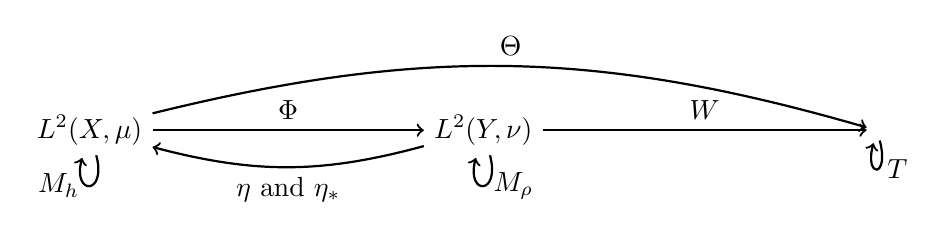
\begin{tikzpicture}[->, thick]
  % Nodes
  \node (A) at (0, 0) {\(L^2(X, \mu)\)};
  \node (B) at (5, 0) {\(L^2(Y, \nu)\)};
  \node (C) at (10, 0) {\(\cH\)};
  % Arrows
  \draw (A) ->  node[above] {\(\Phi\)} (B);
  \draw (B) ->  node[above] {\(W\)} (C);
  \draw (A) to[bend left=15] node[above] {\(\Theta\)} (C);
  % \draw[loop left, min distance=20mm, looseness=8] (A) edge[loop] node[left] {\(M_{h}\)} (A);
  \draw (A) edge[loop below] node[left] {\(M_{h}\)} (A);
  \draw (B) edge[loop below] node[right] {\(M_{\rho}\)} (B);
  \draw (C) edge[loop below] node[right] {\(T\)} (C);
  \draw (B) to[bend left=15] node[below] {\(\eta\) and  \(\eta_*\)} (A);
\end{tikzpicture}
\end{figure}

% \[
% \xymatrix{
%    & \Phi \ar[rrrr] \ar[d] & & & & \mathcal{H} \\
%    M_h \ar@(ul,dl)[] \ar[dr] & L^2(\mathcal{X},\mu') \ar[r]_{\Phi} \ar@/^1pc/[urrrr] & L^2(\mathcal{Y},\nu) \ar[r]^{W} & \mathcal{H} \\
%    & m \ar@/_/[ur] \ar@/_/[rr] & & y^*
% }
% \] 



  \noindent
  First we check the domains, proving \(\Theta \dom(M_{h}) = \dom(T)\):
  
  Let \(f \in \dom(M_{h}) \subset L^2(X, \mu)\). 
  Then \(g \coloneqq (M_{h} + \I) f \in L^2(X, \mu)\). 
  Note, for any \((y, n) \in Y\), that 
  \begin{align*}
    (\Phi g) (y, n) 
    &= \big(\Phi (h + \I) \big)(y, n) (\Phi f)(y, n) \\ 
    &= \Big( h\big(\eta(y), n\big) + \I \Big) (\Phi f)(y, n) = (\eta(y) + \I) (\Phi f) (y, n) . 
  \end{align*}
  Since \(\eta(y) + \I = \I \frac{1 + y}{1 - y} + \I = \frac{2 \I}{1 - y}\), we have \((I - M_{\rho}) \Phi g = 2\I \Phi f\). 
  Applying \(W\) on both sides and using  \(WM_{\rho} = UW\) gives \((I - U) \Theta g = 2 \I \Theta f\). 
  From definition, \(I - U = 2 \I (T + \I)^{-1}\), so 
  \begin{equation}
  \label{eqn:spectral-thm-ast}
    \Theta f = (T + \I)^{-1} \Theta g \in \dom(T) . 
    \tag{\(\ast\)}
  \end{equation}
  It follows that \(\Theta \dom(M_{h}) = \dom(T)\). 

  Next, let \(v \in \dom(T)\) and \(w \coloneqq (T + \I) v\). Then \[
    v = (T + \I)^{-1} w = \frac{1}{2 \I} (I - U) w . 
  \] 
  From \(W^{-1} U W = M_{\rho}\), we have \(I - U = W M_{1 - \rho} W^{-1}\).
  Thus \(W^{-1} v = \frac{1}{2 \I} M_{1 - \rho} W^{-1} w\), and we have 
  \begin{equation}
  \label{eqn:spectral-thm-dagger}
    \Theta^{-1} v = \Phi^{-1} W^{-1} v = \frac{1}{2 \I} \Phi^{-1} M_{1 - \rho} W^{-1} w . 
    \tag{\(\dagger\)}
  \end{equation}
  Now note that for \(g \in L^2(Y, \nu)\) and any \((x, n) \in X\) we have
  % \[
  %   (\Phi^{-1} M_{1 - \rho} g)(x, n) = (M_{1 - \rho} g) \big(c(x), n\big) = \big(1 - c(x)\big) g\big( c(x), n \big) . 
  % \] 
  \begin{align*}
    (\Phi^{-1} M_{1 - \rho} g)(x, n) 
    &= (M_{1 - \rho} g) \big(c(x), n\big) \\
    &= \big(1 - c(x)\big) g\big( c(x), n \big) 
      = \left( 1 - \frac{x - \I}{x + \I} \right) g\big( c(x), n \big) \\ 
    &= \frac{2\I}{x + \I} (\Phi^{-1} g) (x, n) . 
  \end{align*}
  That is, \(\Phi^{-1} M_{1 - \rho} = 2 \I (M_{h} + \I)^{-1} \Phi^{-1}\). Combined with (\ref{eqn:spectral-thm-dagger}) we get 
  \[
    \Theta^{-1} v = (M_{h} + \I)^{-1} \Theta^{-1} w \in \ran\big((M_{h} + \I)^{-1}\big) = \dom(M_{h}) . 
  \] 
  It follows that \(\dom(T) \subset \Theta \dom(M_{h})\), and thus \(\dom(T) = \Theta \dom(M_{h})\). 

  To finish the proof, note that for any \(f \in \dom(M_{h})\), by (\ref{eqn:spectral-thm-ast}), we have \(\Theta (M_{h} + \I) f = (T + \I) \Theta f\).
  This gives \(\Theta M_{h} = T \Theta\). 
\end{proof}





With the spectral theorem, we can now construct a functional calculus for self-adjoint operators. 
For a bounded Borel function \(f \in \cB_\mathrm{b}(\RR): \RR \to \CC\), we define 
\[
  f(T) \coloneqq \Theta M_{f \circ h} \Theta^{-1} 
\] 
where \(\Theta\) and \(h\) are given in \Cref{thm:spectral-thm-self-adjoint}. 
Note that since \(f \circ h\) is bounded, the operator \(f(T)\) is bounded by \Cref{thm:multiplication-operator-adjoint}. 

The map defined above has the following properties:
\begin{proposition}~
\label{thm:self-adjoint-FC}
  Let \(T\) be a self-adjoint operator. 
  % The map 
  % \[
  %   \cB_{\mathrm{b}}(\RR) \to \cL, \quad
  %   f \mapsto f(T) \coloneqq \Theta M_{f \circ h} \Theta^{-1} 
  % \] 
  % has the following properties:
  \begin{enumerate}[label=(\alph*)]
    \item\label{enum:self-adjoint-FC:*homomorphism}
      % It is a \vocab{\(*\)-homomorphism}.
      For any \(f, g \in \cB_{\mathrm{b}}(\RR)\), we have \((fg)(T) = f(T)g(T)\) and \(f(T)^* = \overline{f}(T)\). 
    % \item\label{enum:self-adjoint-FC:}
    %   For any \(f \in \cB_{\mathrm{b}}(\RR)\), there holds
    %   \[
    %     \norm{f(T)} \leq \sup_{\lambda \in \spec T} \abs{f(\lambda)}, 
    %   \] 
    %   with equality if \(f\) is continuous.  
    \item\label{enum:self-adjoint-FC:stronglim}
      Let \(f_{n} \to f\) pointwise and \(\norm{f_{n}}_{\infty} < M\) for each \(n\).
      Then \(f_{n}(T) \to f(T)\) in the strong operator topology, that is, \(f_{n}(T) \to f(T) v\) for all \(v \in \cH\).
      % We denote this type of convergence also as 
      % \[
      %   \lim_{n \to \infty} f_{n}(T) = f(T) . 
      % \] 
      % in the strong sense, i.e., \(f_{n}(T)v \to f(T)v\) for any \(v \in \cH\). 
    % \item for any \(z \in \CC \setminus \RR\) and the functions \(r_z: \RR \ni x \mapsto (x - z)^{-1} \in \CC\) there holds \(r_z(T) = (T - z)^{-1}\). 
  \end{enumerate}
  % Moreover, this map is unique. 
\end{proposition}
\begin{proof}~
  \begin{enumerate}[label=(\alph*)]
  \item % *-homomorphism
    Let \(f, g \in \cB_{\mathrm{b}}(\RR)\). 
    We have
    \[
      f(T) g(T)
      = \Theta M_{f \circ h} M_{g \circ h} \Theta^{-1} 
      = \Theta M_{(fg) \circ h} \Theta^{-1} 
      = (fg) (T) 
    \] 
    and 
    \[
      f(T)^* 
      = \Theta M_{\overline{f \circ h}} \Theta^{-1} 
      = \overline{f}(T) . 
    \] 
  % \item % ||f(T)|| <= sup |f(l)|, where l in spec T; with equality if f is continuous 
  \item % if f_n \to f pointwise and each sup |f| < M, then f_n(T) \to f(T) in the strong sense
    The dominated convergence theorem\footnote{See \cite[p.~55]{bass2014real}. } gives
    \[
      \lim_{n \to \infty} \norm{(f_{n} \circ h - f \circ h) v} 
      = \lim_{n \to \infty} \int_{X} \abs{(f_{n} - f) \circ h}^2 \abs{v}^2 \d\mu
      = 0
    \] 
    for all \(v \in L^2(X, \mu)\). 
    Thus we have \(f_{n}(T)v \to f(T)v\). 
  \end{enumerate}
\end{proof}

We remark that the Spectral Theorem can be used to prove the following result showing the utility of obtaining the spectrum:
\begin{theorem}
  For a self-adjoint operator \(T\) and \(c \in \RR\), we have 
  \begin{enumerate}[label=(\alph*)]
    \item \(T \geq c\) if and only if \(\spec T \subset [c, \infty)\).
    \item \(T\) is bounded with \(\norm{T} \leq c\) if and only if \(\spec T \subset [-c, c]\). 
  \end{enumerate}
\end{theorem}
\begin{proof}
  See \cite[p.~68]{pankrashkin2022spectral}. 
\end{proof}





\section{Spectral Projectors}
\label{sec:spectral-projectors}

\subsection{Orthogonal Projectors}
We first present a quick review of projection operators:

\begin{definition}
  A linear operator \(P\) on \(\cH\) is called a projection operator if \(P\) is idempotent. 
  That is, \(P^2 = P\). 
  A self-adjoint projection operator is called a \vocab{orthogonal projector}. 
\end{definition}

Let \(P\) be an orthogonal projector. 
We have, for any \(v, w \in \cH\), that 
\[
  \left< v - Pv, Pw \right> 
  = \left< v, Pw \right> - \left< v, P^* P w \right>
  % = \left< v, Pw \right> - \left< v, P w \right>
  = 0. 
\] 
That is, for any \(v \in \cH\), we have \((I - P)v \perp \ran(P)\). 
% Conversely, if \(P\) is a projection operator such that \(\ran(I - P) \perp \ran(P)\), then 
% \[
%   \left< Pv, w \right> = \left< Pv, Pw \right> = \left< v, Pw \right>, \quad \forall v, w \in \cH . 
% \] 
% and \(P\) is self-adjoint. 
A similar argument shows that the converse is also true.
That is, we have that a projection operator \(P\) is an orthogonal projector if and only if \(\ran(I - P) \perp \ran(P)\). 

Note also that projection operators do not increase distance; \(\norm{P} \leq 1\).

\begin{lemma}
\label{thm:orthogonal-projections}
  Let \(P_1\) and \(P_2\) be orthogonal projectors on \(\cH\) with \(\ran(P_1) \perp \ran(P_2)\).
  Then \(P_1P_2 = P_2P_1 = 0\) and \(\ran(P_1 + P_2) = \ran(P_1) + \ran(P_2)\). 
\end{lemma}
\begin{proof}
  It is clear that \(\ran(P_1 + P_2) \subset \ran(P_1) + \ran(P_2)\). 
  We prove the opposite inclusion. 
  For any \(v \in \cH\), since \(P_2v \perp \ran(P_1)\), we have \(P_1P_2v = 0\). 
  Similarly, \(P_2P_1 \equiv 0\). 
  Now, pick any \(v \in \ran(P_1) + \ran(P_2)\).
  Then \(v = P_1 w_1 + P_2 w_2\) for some \(w_1\) and \(w_2\) in \(\cH\).  
  From above, 
  \[
    (P_1 + P_2)(P_1w_1 + P_2w_2)
    = P_1^2 w_1 + P_2^2 w_2
    = P_1w_1 + P_2 w_2
    = v.
  \] 
  Thus \(v \in \ran(P_1 + P_2)\). 
\end{proof}

% \begin{lemma}
%   Let \((P_n)\) be a sequence of increasing orthogonal projectors on \(\cH\), that is,  \(\ran(P_n) \subseteq \ran(P_{n + 1})\) for all \(n\). 
%   Then \(P \coloneqq \lim_{n \to \infty} P_n\) is the orthogonal projector on \(\overline{\bigcup_{n = 1}^{\infty} \ran(P_n)}\). 
% \end{lemma}
% \begin{proof}
%   Let \(1 \leq n \leq m\) be arbitrary. 
%   Note, first, that since \(\ran(P_n) \subseteq \ran(P_{m})\), we have \(P_{m} P_n = P_n\) and, by taking the adjoints on both sides, \(P_n P_{m} = P_{n}\). 
%   Then, for each \(u \in \cH\), we have 
%   \[
%   \norm{P_n u}^2
%   = \norm{P_n P_{n + 1} u}^2
%   \leq \norm{P_{n + 1} u}^2. 
%   \] 
%   As each \(\norm{P_n} \leq 1\), this gives the convergence of \((\norm{P_n u})\). 

%   Next, from 
%   \[
%     \left< P_{n + 1} u, P_n u \right> 
%     = \norm{P_n u} 
%     = \left< P_{n} u, P_{n + 1} u \right> 
%   \]
%   we have
%   \[
%     \norm{(P_{n + 1} - P_n) u}
%     % = \left< (P_{n + 1} - P_n) u, (P_{n + 1} - P_n) u \right>
%     = \norm{P_{n + 1} u}  - \norm{P_n u} 
%     \longrightarrow 0. 
%   \] 
%   Thus \(P\) exists and is bounded. 
%   We next verify that \(P\) is an orthogonal projector:

%   By each \(P_n\) being self-adjoint, we have for all \(u, v \in \cH\) that 
%   \[
%     \left< v, Pu \right> 
%     = \lim_{n \to \infty} \left< v, P_n u \right>
%     = \lim_{n \to \infty} \left< P_n v, u\right>
%     = \left< Pv, u \right> . 
%   \] 
%   This shows that \(P\) is self-adjoint.
%   To show that \(P\) is idempotent, note that for any \(u \in \cH\), we have
%   \[
%   P^2(u)
%   = \lim_{n \to \infty} P_n \left( \lim_{m \to \infty} P_m u \right) 
%   = \lim_{n \to \infty} \lim_{m \to \infty} P_n P_m u
%   = \lim_{n \to \infty} P_n u
%   = P u . 
%   \] 

%   Finally, we verify the range.
%   By above, for each \(u\), we have \(\norm{P_n u - Pu} \to 0\), where each \(P_n u \in \ran(P_n)\).
%   This gives \(\ran(P) \subset \overline{\bigcup_{n = 1}^{\infty} \ran(P_n)}\). 
%   To see the opposite inclusion, note that \(P_m\big(\ran(P_n)\big) = \ran(P_n)\) for all \(m > n\). 
%   By sending \(m\) to infinity, we have \(\ran(P_n) \subset \ran(P)\) for each \(n\). 
%   Noting that as a bounded operator, \(P\) has closed range, we have \(\overline{\bigcup_{n = 1}^{\infty} \ran(P_n)} \subset \ran(P)\).
% \end{proof}


\subsection{Spectral Resolution}
Applying indicator functions on Borel sets to self-adjoint operators gives a family of orthogonal projectors:

\begin{definition*}
  Let \(E \subset \RR\) be a Borel subset and \(T\) a self-adjoint operator. 
  The \vocab{spectral projector} of \(T\) on \(E\) is the orthogonal operator \(P(E) \coloneqq \ind_{E}(T)\). 
\end{definition*}

The mapping \(E \mapsto P(E)\) is called the \vocab{spectral resolution} of \(T\) and can be understood as a \vocab{projection-valued measure} with support \(\spec T\).
Additivity holds since disjoint Borel sets are mapped to mutually orthogonal projection operators, that is, projection operators with mutually orthogonal images (recall \Cref{thm:orthogonal-projections}). 

One may think of the range of \(P(E)\), where \(E\) is a Borel subset of \(\RR\), as the part of the Hilbert space governed only by \(E\), independent of the other parts of the spectrum.
As we will see, the range of the projector \(P \{\lambda\}\) is always the nullspace of \(T - \lambda\). 
Thus, when \(\lambda\) is an eigenvalue, we have \(T u = \lambda u\) for any \(u\) in the eigenspace \(\ran(P \{\lambda\}) = \ker(T - \lambda)\). 
One may thus express a self-adjoint operator \(T\) on an infinite dimensional Hilbert space as 
\[
  Tu = \int_{\spec T} \lambda \dd P(\d\lambda) u . 
\] 
This is analogous to the finite dimensional case, where we have 
\[
  T u = \sum_{n=1}^{N} \lambda_n P_n , 
\] 
where operators \(P_n\) project onto the eigenspaces associated with \(\lambda_n\). 


This can be made rigorous. 
For our purpose, though, it suffices to view \(P(\cdot)\) as orthogonal projectors and establish its finite additivity.



\begin{proposition}
\label{thm:SP}
  Let \(T\) be a self-adjoint operator in \(\cH\), \(P\) the spectral resolution of \(T\), and \(E, F \subset \RR\) disjoint Borel sets. 
  Then 
  \begin{enumerate}[label=(\alph*)]
    \item\label{enum:SP-prop:orthogonality} 
      \(P(E)\) is an orthogonal projector, 
    \item\label{enum:SP-prop:identity} 
      \(P(\emptyset) = 0\) and \(P(\RR) = I\), 
    \item\label{enum:SP-prop:additivity} 
      % \(\ran(P(E)) \perp \ran(P(F))\) and 
      \(P(E \cup F) = P(E) + P(F)\) has range \(\ran\big(P(E \cup F)\big) = \ran\big(P(E)\big) + \ran\big(P(F)\big)\), 
    \item\label{enum:SP-prop:supp} 
    \(P(a, b) = 0\)\footnotemark if and only if \(\spec T \cap (a, b) = \emptyset\), 
    \item\label{enum:SP-prop:range} 
      \(\ran(P\{\lambda\}) = \ker\big( T - \lambda \big)\) for any \(\lambda \in \RR\).
  \end{enumerate}
\end{proposition}
\begin{proof}
  % It is easy to check that operators unitarily equivalent to orthogonal projectors are orthogonal projectors, so 
  We assume \(\cH = L^2(X, \mu)\) and \(T = M_h\) with \(X, \mu, h\) as in \Cref{thm:spectral-thm-self-adjoint}. 
  Thus we have \(P(E) = M_{\ind_{E} \circ h}\). 
  It is easy to check that the same statements hold for any operator \(T\) unitarily equivalent to \(M_{h}\). 
  \begin{enumerate}[label=(\alph*)]
  \item % P(E) is an orthogonal projector 
    Since \(\ind_{E}\) is idempotent, we have 
    \[
      P(E)^2
      = \left( M_{\ind_{E} \circ h} \right)^2
      = M_{\ind_{E}^2 \circ h}
      = M_{\ind_{E} \circ h}
      = P(E) . 
    \] 
    Similarly, since \(\ind_{E}\) is real-valued, by \Cref{thm:multiplication-operator-adjoint} we have \(P(E)^* = P(E)\). 

  \item % P(\emptyset) = 0l P(\RR) = I
    Note that \(\ind_{\emptyset} \circ h \equiv 0\) and \(\ind_{\RR} \circ h \equiv 1\). 

  \item % finite additivity; P(E \cup F) = P(E) + P(F)
    The first statement follows from \(\ind_{E \cup F} = \ind_{E} + \ind_{F}\). 
    To show the second statement, by \Cref{thm:orthogonal-projections}, we need only show \(\ran\big(P(E)\big) \perp \ran\big(P(F)\big)\):

    Let \(u \in \ran(P(E))\) and \(v \in \ran(P(F))\). 
    By \ref{enum:SP-prop:orthogonality}, we have \(u = (\ind_{E} \circ h) u\). 
    Thus, \(u(x) = 0\) for all  a.e.\ \(x \not\in E\). 
    Similarly, \(v(x) = 0\) for all a.e.\ \(x \not\in F\). 
    Since \(E \cap F = 0\), we have  \(\left< u, v \right> = 0\). 

  \item % supp; P(a, b) = 0 iff \spec T \cap (a, b) = \emptyset
    The condition \(P\big((a, b)\big) = 0\), that is, \(\ind_{(a, b)} \circ h = 0\) a.e., is equivalent to \((a, b) \cap \essran h = \emptyset\), and \(\essran h = \spec M_{h}\) by \Cref{thm:multiplication-operator-spectrum}. 

  \item % \ran(P {l}) = \ker(T - l)
    Let \(u \in L^2(X, \mu)\). 
    The condition \((h - \lambda) u = 0\) is equivalent to \(u = 0\) a.e.\ when \(h - \lambda \neq 0\). 
    This happens if and only if \(u = (\ind_{\{\lambda\}} \circ h) u = P\{\lambda\} u\), which means precisely \(u \in \ran(P \{\lambda\})\) since \(P \{\lambda\}\) is an orthogonal projector. 
  \end{enumerate}
\end{proof}


By analyzing spectral projectors associated with different Borel sets, we can isolate the effect of different parts of the spectrum. 
Bounds of these Borel sets enable us to create useful estimates: 

\begin{proposition}
\label{thm:SP2}
  Let \(T\) and \(P\) be as above, and \(\lambda \in \RR\). 
  \begin{enumerate}[label=(\alph*)]
    \item\label{enum:SP-prop:1} 
      Let \(P_{\epsilon} \coloneqq P(\lambda - \epsilon, \lambda + \epsilon)\). 
      Then for all \(v \in \ran(P_{\epsilon}) \subset \dom(T)\) we have 
      % Then \(\ran(P_{\epsilon}) \subset \dom(T)\) and for all \(v \in \ran(P_{\epsilon}) \subset \dom(T)\) we have 
      \[
        \norm{(T - \lambda) v} \leq \epsilon . 
      \] 
      % \(\ran\big(P(\lambda - \epsilon, \lambda + \epsilon)\big) \subset \dom(T)\) and 
      % \(\norm{(T - \lambda) v} \leq \epsilon\) for all \(v \in \ran\big(P(\lambda - \epsilon, \lambda + \epsilon)\big)\); 
    \item\label{enum:SP-prop:2} 
      % Let \(v \in \dom(T) \cap \ran\big(P[\lambda, \infty)\big)\). 
      Let \(v \in P[\lambda, \infty) \dom(T)\).
      Then 
      \[
        \left< v, Tv \right> \geq \lambda \norm{v}^2 . 
      \] 
    % \item \label{enum:SP-prop:s-lim}
    %   \(P(\lambda - \epsilon, \lambda + \epsilon)\) converges to \(P \{\lambda\}\) pointwise as \(\epsilon \to 0^+\). 
      % \(P \{\lambda\} = \stronglim_{\epsilon \to 0^+} P(\lambda - \epsilon, \lambda + \epsilon)\) 
      % That is, 
      % \[
      % P \{\lambda\}u = \lim_{\epsilon \to 0^+} P(\lambda - \epsilon, \lambda + \epsilon) u
      % \] 
      % for any \(u \in \cH\). 
  \end{enumerate}
\end{proposition}
\footnotetext{We write \(P(a, b) = P((a, b))\) for clarity. }
\begin{proof}
  Again, we assume \(\cH = L^2(X, \mu)\) and \(T = M_{h}\), with  \(X\), \(\mu\), and \(h\) as in \Cref{thm:spectral-thm-self-adjoint}. 
  \begin{enumerate}[label=(\alph*)]
  \item 
    Let \(u \in L^2(X, \mu)\) and \(v \coloneqq P_{\epsilon} u = (\ind_{(\lambda - \epsilon, \lambda + \epsilon)} \circ h) u\). 
    We check first that \(v \in \dom(T)\): 

    When \(x \not\in (\lambda - \epsilon, \lambda + \epsilon)\) we have \(v = \ind_{(\lambda - \epsilon, \lambda + \epsilon)} \circ h = 0\). 
    Thus, for all \(v \neq 0\), there holds \(x \in (\lambda - \epsilon, \lambda + \epsilon)\) and then \(\abs{h} \leq \abs{\lambda} + \epsilon\). 
    We then have 
    \[
      \int_{X} \abs{h v}^2 \dd\mu
      \leq \int_{\{x \in X: v(x) \neq 0\}} \big(\abs{\lambda} + \epsilon\big)^2 \abs{v}^2 \dd\mu 
      = \big(\abs{\lambda} + \epsilon\big)^2 \norm{v}^2 < \infty . 
    \] 
    This gives \(v \in \dom(M_{h})\). 

    Similarly, for all \(v \neq 0\), from \(x \in (\lambda - \epsilon, \lambda + \epsilon)\) we know \(\abs{h - \lambda} \leq \epsilon\).
    The estimate then follows:
    \[
      \norm{(M_{h} - \lambda) v}^2
      % = \int_{X} \abs{h - \lambda}^2 \abs{v}^2 \dd\mu
      \leq \int_{\{x \in X: v(x) \neq 0\}} \epsilon^2 \abs{v}^2 \dd\mu  
      = \epsilon^2 \norm{v}^2  
      \leq \epsilon^2 \norm{u}^2 . 
    \] 
    
  \item 
    Let \(u \in \dom(M_{h})\) and \(v \coloneqq P[\lambda, \infty)u = (\ind_{[\lambda, \infty)} \circ h) u\). 
    As above, we have \(v = \ind_{[\lambda, \infty)} \circ h = 0\) for all \(x < \lambda\), and thus \(h \geq \lambda\) when \(v \neq 0\).
    Therefore, 
    \[
      \left< v, M_{h} v \right>
      = \int_{X} h \abs{v}^2 \dd\mu 
      \geq \int_{\{x \in X: v(x) \neq 0\}} \lambda \abs{v}^2 \dd\mu
      = \lambda \norm{v}^2 . 
    \] 
%   \item 
%     This follows from the fact that \(\ind_{(\lambda - \epsilon, \lambda + \epsilon)}\) converges to \(\ind_{\{\lambda\}}\) pointwise as \(\epsilon \to 0^+\).
  \end{enumerate}
\end{proof}




\subsection{Discrete and Essential Spectrum}

\begin{definition}
  Let \(T\) be a self-adjoint operator in \(\cH\). 
  The \vocab{discrete spectrum} \(\discspec T\) is the set of \(\lambda \in \spec T\) such that \(P(\lambda - \epsilon, \lambda + \epsilon)\) has infinite rank for all \(\epsilon > 0\). 
  The \vocab{essential spectrum} of \(T\) is defined as
  \[
    \essspec T \coloneqq \spec T \setminus \discspec T.
  \]
\end{definition}

\begin{proposition}
  Let \(T\) be a self-adjoint operator in \(\cH\). 
  A complex number \(\lambda\) is in the discrete spectrum of \(T\) if and only if \(\lambda\) is an eigenvalue of \(T\) of finite multiplicity and an isolated point of \(\spec T\) (such eigenvalues are called \vocab{discrete eigenvalues}). 
\end{proposition}
\begin{proof}
  Let \(\lambda \in \discspec T\). 
  By \Cref{thm:SP} and definition of the discrete spectrum, there exists some \(\epsilon_0 > 0\) such that \(N \coloneqq \dim \ran\big(P(\lambda - \epsilon_0, \lambda + \epsilon_0)\big)\) is finite and nonzero. 
  Now, note that the function
  \[
  (0, \epsilon_0) \longrightarrow \{1, \cdots, N\}, 
  \quad \epsilon \longmapsto P(\lambda - \epsilon, \lambda + \epsilon). 
  \] 
  is nondecreasing (recall the partial ordering of self-adjoint operators; see \Cref{def:self-adjoint-partial-ordering}). 
  There, thus, exists a \(\epsilon_1 \in (0, \epsilon_0)\) such that \(P_1 \coloneqq P(\lambda - \epsilon, \lambda + \epsilon)\) is constant for all \(\epsilon\) in the interval \((0, \epsilon_1) \subset (0, \epsilon_0)\). 
  We then have by \Cref{thm:self-adjoint-FC} \ref{enum:self-adjoint-FC:stronglim} that 
  \[
    P(\lambda - \epsilon, \lambda + \epsilon) \equiv P_1 \longrightarrow P \{\lambda\}
  \]
  in the strong operator topology as \(\epsilon \to 0^+\). 
  This gives \(P_1 = P \{\lambda\}\). 
  Thus \(\ran(P \{\lambda\}) = \ran(P_1) > 0\) and \(\lambda \in \pspec T\). 
  % To see that \(\lambda\) is an isolated point of the spectrum, 
  Next, choose a fixed \(\epsilon_2 \in (0, \epsilon_1)\) and note that 
  \[
    P \{\lambda\} = P_1 = P(\lambda - \epsilon_2, \lambda + \epsilon_2) . 
  \] 
  Thus the spectrum is empty in \((\lambda - \epsilon_2, \lambda) \cup (\lambda, \lambda + \epsilon_2)\). 
  That is, \(\lambda\) is an isolated point of the spectrum. 


  Conversely, let \(\lambda\) be an eigenvalue of finite multiplicity and an isolated point of the spectrum. 
  Then there exists \(\epsilon > 0\) such that the spectrum is empty in \((\lambda - \epsilon, \lambda) \cup (\lambda, \lambda + \epsilon)\). 
  Thus 
  \[
    \dim\ran\big(P(\lambda - \epsilon, \lambda + \epsilon)\big) = \dim\ran\big(P \{\lambda\} \big) < \infty . 
  \] 
\end{proof}






\section{The Min-Max Theorem}
\label{sec:min-max}


The min-max theorem gives a variational characterization to the discrete eigenvalues below the essential spectrum, relating them to the \vocab{Rayleigh quotient} \(\frac{\left< u, Tu \right>}{\left< u, u \right>}\), which one may think of as a measure of how much \(T\) stretches \(u\) in the direction of \(u\) itself.
Given the constraint \(u \in W\), where \(W\) is a one dimensional subspace, we can then expect the Rayleigh quotient to be maximized when \(u\) is in the eigenspace contained in \(W\) that is associated with the largest eigenvalue, and taking the minimum over all possible constraints \(W\) gives the lowest eigenvalue. 
Larger eigenvalues can then be obtained by increasing the dimension of \(W\) to filter out smaller ones.
This provides the intuition for the following:
% \todo{is this intuition right?}


% Let \(T\) be a lower semi-bounded\todo{add why} self-adjoint operator in an infinite-dimensional Hilbert space \(\cH\). We denote \[
%   \Sigma \coloneqq 
%   \begin{cases}
%     \inf \essspec T, & \text{if} \essspec T \neq \emptyset, \\
%     +\infty, & \text{otherwise}. 
%   \end{cases}
% \] 

\begin{theorem}[Min-Max Theorem]
  Let \(T\) be a self-adjoint operator whose spectrum is bounded below. 
  Let \(\Lambda_k\) denote the set of subspaces of \(\dom(T)\) of dimension \(k\) and define 
  \[
    \alpha_k \coloneqq \inf_{W \in \Lambda_k} \sup_{u \in W \setminus \{0\}} \frac{\left< u, Tu \right>}{\left< u, u \right>} 
  \] 
  for \(k \in \NN\). 

  Then the sequence \((\alpha_k)\) is non-decreasing, and for each \(k\), one and only one of the following holds:
  \begin{enumerate}[label=(\alph*)]
    \item \(\alpha_k\) is the \(k\)th eigenvalue (arranged in increasing order and counted with multiplicity) and there are at least \(k\) eigenvalues below the essential spectrum. 
    \item \(\alpha_k = \inf \essspec T\) and there are at most \(k - 1\) eigenvalues below the essential spectrum. 
  \end{enumerate}
\end{theorem}
\begin{proof}
  For any \(n\), we have (think adding and relaxing constraints)
  \[
    \inf_{W \in \Lambda_{n + 1}} \sup_{u \in W \setminus \{0\}} \frac{\left< u, Tu \right>}{\left< u, u \right>} 
    \geq \inf_{W \in \Lambda_{n + 1}} \inf_{\substack{V \in \Lambda_n\\ V\subset W}} \sup_{u \in V \setminus \{0\}} \frac{\left< u, Tu \right>}{\left< u, u \right>} 
    \geq \inf_{V \in \Lambda_n} \sup_{u \in V \setminus \{0\}} \frac{\left< u, Tu \right>}{\left< u, u \right>} . 
  \]
  So the sequence \((\alpha_n)\) is non-decreasing. 

  Next, let \(\Sigma \coloneqq \inf \essspec T\) (set \(\Sigma \coloneqq \infty\) if \(\essspec T\) is empty).
  Denote the \(k\)th eigenvalue (counting multiplicities) in \((-\infty, \Sigma)\) by \(E_k\) and the associated eigenvector \(\phi_k\), where \(k \in \{1, \cdots, N\}\) with \(N \in \NN \cup \{\infty\}\). 
  By \Cref{thm:self-adjoint-spectrum}, we may assume that the set of \(\phi_k\) form an orthonormal family. 
  Let \(V_n \coloneqq \Span \{\phi_1, \cdots, \phi_n\} \in \Lambda_n\).
  For any \(u \in V_n\), there holds
  \begin{align*}
    \left< u, Tu \right>
    = \left< \sum_{j=1}^{n} \left< \phi_j, u \right> \phi_j, \sum_{j=1}^{n} \left< \phi_j, u \right> E_j \phi_j \right>
    = \sum_{j=1}^{n} E_j \abs{\left< \phi_j, u \right>}^2 
    \leq E_n \sum_{j=1}^{n} \abs{\left< \phi_j, u \right>}^2 
    =  E_n \norm{u}^2 . 
  \end{align*}
  Thus, \(\alpha_n \leq E_n\). 

  To prove the opposite inequality, let \(W \in \Lambda_n\) and \(P\) the orthogonal projector on the subspace \(\Span \{E_1, \cdots, E_{n - 1}\}\). 
  From \Cref{thm:SP}, we know that 
  \[
    \ran\big(P(-\infty, E_n)\big) \subset \ran(P) \leq n - 1 < \dim W. 
  \]
  Thus we can always find a \(v \in W \setminus \{0\}\) such that \(P v = 0\). 
  Since \(P\) is an orthogonal projector, we have \(v \in \ran\big(P(-\infty, E_n)\big)\) and thus \(v \in \ran\big(P[E_n, \infty)\big)\). 
  \Cref{thm:SP2} then gives 
  \[
    \sup_{u \in W \setminus \{0\}} \frac{\left< u, T u \right>}{\left< u, u \right>}
    \geq \frac{\left< v, Tv \right>}{\left< v, v \right>}
    \geq E_n. 
  \] 
  Thus we have \(\alpha_n = E_n\). 

  Now, if \(N = \infty\), the proof is complete. 
  Otherwise, it remains to show \(\alpha_n = \Sigma\) for all \(n \geq N + 1\): 

  From \Cref{thm:SP}, we have \(P(-\infty, \Sigma) = \sum P \{E_j'\}\), where \(E_j\) are distinct eigenvalues in \((-\infty, \Sigma)\). 
  Since \(\ran\big(P \{E_j'\} \big)\) are distinct, mutually orthogonal eigenspaces, we have 
  \[
    \dim \ran\big(P(-\infty, \Sigma)\big)
    = \sum \dim \ran\big(P\{E_j'\}\big)
    = N .
  \] 
  Let \(n \geq N + 1\) and \(W \in \Lambda_{n}\). 
  Then there exists a \(v \in W \setminus \{0\}\) such that \(v \perp \ran\big(P(-\infty, \Sigma)\big)\) and a similar argument as above shows that \(\alpha_n \geq \Sigma\). 

  To prove the opposite inequality, consider \(W \coloneqq \ran\big(P(\Sigma - \epsilon, \Sigma + \epsilon)\big)\) with \(\epsilon > 0\). 
  Since \(\Sigma = \inf \essspec T\), this is an infinite dimensional subspace. 
  Let \((e_j)_{j \in \NN}\) be an orthonormal basis of \(W\) and set \(W_n \coloneqq \Span \{e_1, \cdots, e_n\}\).
  We then have, by \Cref{thm:SP2} \ref{enum:SP-prop:1}, 
  \[
    \left< u, Tu \right> - \Sigma \norm{u}^2  
    \leq \abs{\left< u, (T - \Sigma)u \right>} 
    \leq \norm{u} \norm{(T - \Sigma)u} 
    \leq \epsilon \norm{u}^2 
  \] 
  for any \(u \in W_n\). 
  This gives \(\left< u, Tu \right> \leq (\Sigma + \epsilon) \norm{u}^2 \) and thus
  \[
    \alpha_n \leq \sup_{u \in W_n, u \neq 0} \frac{\left< u, Tu \right>}{\left< u, u \right>} \leq \Sigma + \epsilon . 
  \] 
  We complete the proof by sending \(\epsilon\) to \(0\). 
\end{proof}







\section*{Acknowledgments}
I am grateful to Andreas Stavrou for reigniting my passion for mathematics in MATH160s, and to Professor Peter May for allowing me to change my decision about writing a paper.
% I am grateful to Professor Peter May for allowing me to change my decision about writing a paper, even after the program had already begun. 
% I sincerely thank Andreas Stavrou for an inspiring year in MATH160s, which reignited my passion for mathematics. 
I am deeply indebted to my mentor, DeVon Ingram, whose patience and guidance helped me realize that I am sometimes able to grasp mathematical concepts that intimidated me. 
% Lastly, my sincere thanks to AZ, HW, RD, and WC for unwavering support and shared laughter, and Zane Miller for his existence. 
Lastly, my sincere thanks to Alexandra Zhou, Hanlei Wen, Ryan Dai, Will Comess, and Joshua Johnson for unwavering support and shared laughter. 
% for unwavering support and the laughter we enjoyed, and Zane Miller for his existence. 





\printbibliography
\nocite{*}


\end{document}




